\documentclass[11pt]{article}
\usepackage[margin=1.0in]{geometry}
\usepackage{setspace}
\usepackage{amsmath}
\usepackage{fancyhdr}
\usepackage{listings}
\usepackage{tikz}
\pagestyle{fancy}
\lhead{CS 4610 Written Assignment 1}
\rhead{Zihao Wang (zw2rf)}
\cfoot{\thepage}
\renewcommand{\headrulewidth}{0.4pt}
\renewcommand{\footrulewidth}{0.4pt}
\begin{document}
\thispagestyle{empty}
\title{CS 4610 Written Assignment 1}
\author{Zihao Wang (zw2rf)}
\date{\today}
\maketitle
\doublespacing

\section{For each of the follow prompts, write any non-empty sentence}
\begin{itemize}
\item I would like to learn the advantages of functional languages. Also, I want to learn why different languages have so different syntaxes and grammars. 
\item Did Professor Weimer learn linguistics before?
\end{itemize}

\section{Consider the following languages over the alphabet $\Sigma = \{a, b\}$}
\begin{center}
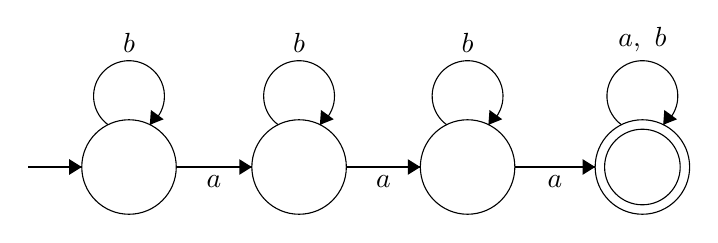
\begin{tikzpicture}[scale=0.2]
\tikzstyle{every node}+=[inner sep=0pt]
\draw [black] (33.9,-27.9) circle (3);
\draw [black] (44.6,-27.9) circle (3);
\draw [black] (55.7,-27.9) circle (3);
\draw [black] (55.7,-27.9) circle (2.4);
\draw [black] (23.1,-27.9) circle (3);
\draw [black] (36.9,-27.9) -- (41.6,-27.9);
\fill [black] (41.6,-27.9) -- (40.8,-27.4) -- (40.8,-28.4);
\draw (39.25,-28.4) node [below] {$a$};
\draw [black] (47.6,-27.9) -- (52.7,-27.9);
\fill [black] (52.7,-27.9) -- (51.9,-27.4) -- (51.9,-28.4);
\draw (50.15,-28.4) node [below] {$a$};
\draw [black] (26.1,-27.9) -- (30.9,-27.9);
\fill [black] (30.9,-27.9) -- (30.1,-27.4) -- (30.1,-28.4);
\draw (28.5,-28.4) node [below] {$a$};
\draw [black] (16.7,-27.9) -- (20.1,-27.9);
\fill [black] (20.1,-27.9) -- (19.3,-27.4) -- (19.3,-28.4);
\draw [black] (32.577,-25.22) arc (234:-54:2.25);
\draw (33.9,-20.65) node [above] {$b$};
\fill [black] (35.22,-25.22) -- (36.1,-24.87) -- (35.29,-24.28);
\draw [black] (43.277,-25.22) arc (234:-54:2.25);
\draw (44.6,-20.65) node [above] {$b$};
\fill [black] (45.92,-25.22) -- (46.8,-24.87) -- (45.99,-24.28);
\draw [black] (54.377,-25.22) arc (234:-54:2.25);
\draw (55.7,-20.65) node [above] {$a,\mbox{ }b$};
\fill [black] (57.02,-25.22) -- (57.9,-24.87) -- (57.09,-24.28);
\draw [black] (21.777,-25.22) arc (234:-54:2.25);
\draw (23.1,-20.65) node [above] {$b$};
\fill [black] (24.42,-25.22) -- (25.3,-24.87) -- (24.49,-24.28);
\end{tikzpicture} \\
$L_{1}$: All strings that contain at least three a's
\end{center} 
\begin{center}
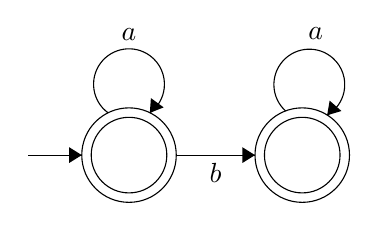
\begin{tikzpicture}[scale=0.2]
\tikzstyle{every node}+=[inner sep=0pt]
\draw [black] (23.1,-27.9) circle (3);
\draw [black] (23.1,-27.9) circle (2.4);
\draw [black] (34.1,-27.9) circle (3);
\draw [black] (34.1,-27.9) circle (2.4);
\draw [black] (16.7,-27.9) -- (20.1,-27.9);
\fill [black] (20.1,-27.9) -- (19.3,-27.4) -- (19.3,-28.4);
\draw [black] (26.1,-27.9) -- (31.1,-27.9);
\fill [black] (31.1,-27.9) -- (30.3,-27.4) -- (30.3,-28.4);
\draw (28.6,-28.4) node [below] {$b$};
\draw [black] (21.777,-25.22) arc (234:-54:2.25);
\draw (23.1,-20.65) node [above] {$a$};
\fill [black] (24.42,-25.22) -- (25.3,-24.87) -- (24.49,-24.28);
\draw [black] (33.052,-25.102) arc (228.26907:-59.73093:2.25);
\draw (34.96,-20.6) node [above] {$a$};
\fill [black] (35.68,-25.37) -- (36.59,-25.1) -- (35.84,-24.44);
\end{tikzpicture} \\
$L_{2}$: All strings that contain at most one b
\end{center} 

\begin{center}
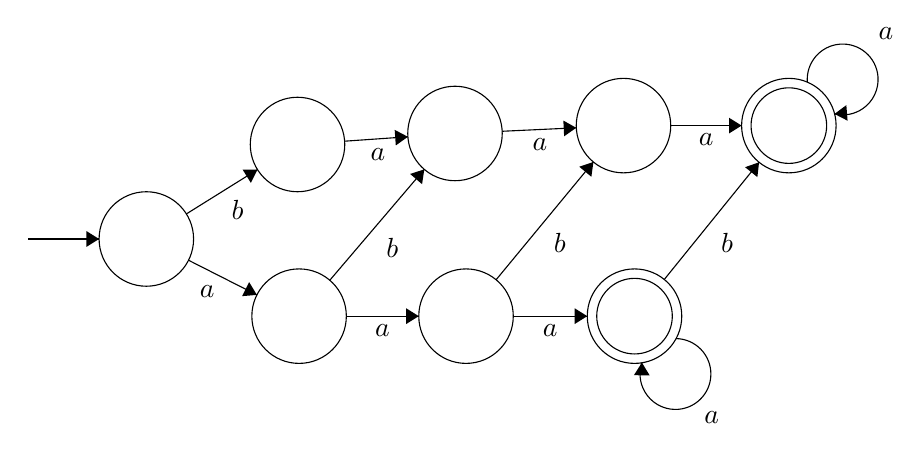
\begin{tikzpicture}[scale=0.2]
\tikzstyle{every node}+=[inner sep=0pt]
\draw [black] (13.4,-25.4) circle (3);
\draw [black] (23,-19.4) circle (3);
\draw [black] (33,-18.7) circle (3);
\draw [black] (23.1,-30.3) circle (3);
\draw [black] (33.7,-30.3) circle (3);
\draw [black] (44.4,-30.3) circle (3);
\draw [black] (44.4,-30.3) circle (2.4);
\draw [black] (43.7,-18.2) circle (3);
\draw [black] (54.2,-18.2) circle (3);
\draw [black] (54.2,-18.2) circle (2.4);
\draw [black] (15.94,-23.81) -- (20.46,-20.99);
\fill [black] (20.46,-20.99) -- (19.51,-20.99) -- (20.04,-21.84);
\draw (19.2,-22.9) node [below] {$b$};
\draw [black] (25.99,-19.19) -- (30.01,-18.91);
\fill [black] (30.01,-18.91) -- (29.17,-18.47) -- (29.24,-19.46);
\draw (28.1,-19.61) node [below] {$a$};
\draw [black] (16.08,-26.75) -- (20.42,-28.95);
\fill [black] (20.42,-28.95) -- (19.93,-28.14) -- (19.48,-29.03);
\draw (17.26,-28.35) node [below] {$a$};
\draw [black] (26.1,-30.3) -- (30.7,-30.3);
\fill [black] (30.7,-30.3) -- (29.9,-29.8) -- (29.9,-30.8);
\draw (28.4,-30.8) node [below] {$a$};
\draw [black] (36.7,-30.3) -- (41.4,-30.3);
\fill [black] (41.4,-30.3) -- (40.6,-29.8) -- (40.6,-30.8);
\draw (39.05,-30.8) node [below] {$a$};
\draw [black] (36,-18.56) -- (40.7,-18.34);
\fill [black] (40.7,-18.34) -- (39.88,-17.88) -- (39.93,-18.88);
\draw (38.39,-18.99) node [below] {$a$};
\draw [black] (46.7,-18.2) -- (51.2,-18.2);
\fill [black] (51.2,-18.2) -- (50.4,-17.7) -- (50.4,-18.7);
\draw (48.95,-18.7) node [below] {$a$};
\draw [black] (5.9,-25.4) -- (10.4,-25.4);
\fill [black] (10.4,-25.4) -- (9.6,-24.9) -- (9.6,-25.9);
\draw [black] (46.29,-27.97) -- (52.31,-20.53);
\fill [black] (52.31,-20.53) -- (51.42,-20.84) -- (52.2,-21.47);
\draw (49.86,-25.68) node [right] {$b$};
\draw [black] (25.05,-28.02) -- (31.05,-20.98);
\fill [black] (31.05,-20.98) -- (30.15,-21.27) -- (30.91,-21.92);
\draw (28.6,-25.94) node [right] {$b$};
\draw [black] (35.61,-27.99) -- (41.79,-20.51);
\fill [black] (41.79,-20.51) -- (40.89,-20.81) -- (41.66,-21.45);
\draw (39.25,-25.68) node [right] {$b$};
\draw [black] (55.374,-15.452) arc (184.60129:-103.39871:2.25);
\draw (59.87,-12.36) node [right] {$a$};
\fill [black] (57.1,-17.46) -- (57.93,-17.89) -- (57.85,-16.9);
\draw [black] (47.027,-31.724) arc (89.28312:-198.71688:2.25);
\draw (49.3,-36.31) node [below] {$a$};
\fill [black] (44.87,-33.25) -- (44.36,-34.05) -- (45.36,-34.06);
\end{tikzpicture} \\
$L_{3}$: All strings that contain at least three a's but at most one b 
\end{center}
\begin{center}
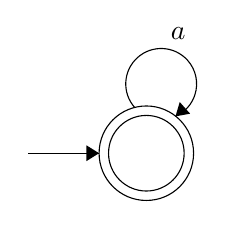
\begin{tikzpicture}[scale=0.2]
\tikzstyle{every node}+=[inner sep=0pt]
\draw [black] (32.8,-29.2) circle (3);
\draw [black] (32.8,-29.2) circle (2.4);
\draw [black] (25.3,-29.2) -- (29.8,-29.2);
\fill [black] (29.8,-29.2) -- (29,-28.7) -- (29,-29.7);
\draw [black] (32.068,-26.303) arc (221.90524:-66.09476:2.25);
\draw (34.82,-22.02) node [above] {$a$};
\fill [black] (34.65,-26.86) -- (35.58,-26.69) -- (34.92,-25.95);
\end{tikzpicture} \\
$L_{4}$: All strings that contain no b's
\end{center}

\section{Give a one-sentence description of the language recognized by the DFA. Write a regular expression for the same language.}
All strings that contain $n$ b's where $n - 3$ is a multiple of 4.\\
The corresponding regular expression in Python is: \lstinline|(a*b){3}((a*b){4})*|

\section{Give a non-deterministic finite automaton (NFA) for the languages}
\begin{center}
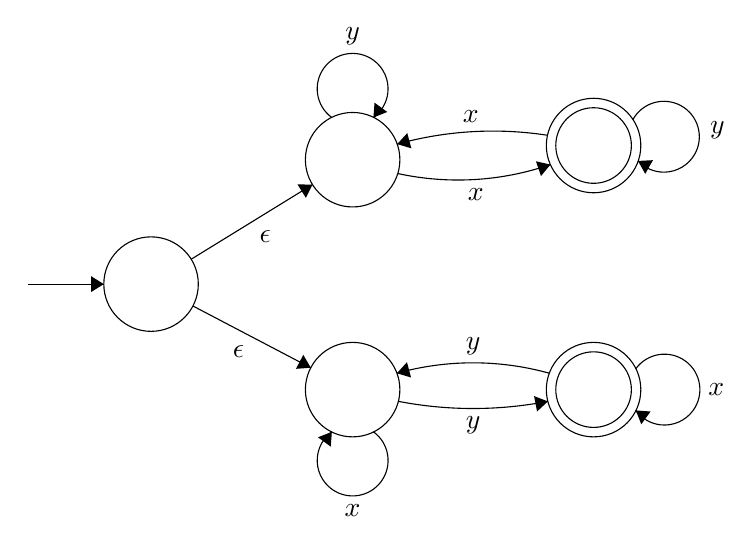
\begin{tikzpicture}[scale=0.2]
\tikzstyle{every node}+=[inner sep=0pt]
\draw [black] (16.5,-28.6) circle (3);
\draw [black] (29.3,-20.7) circle (3);
\draw [black] (29.3,-35.3) circle (3);
\draw [black] (44.6,-19.8) circle (3);
\draw [black] (44.6,-19.8) circle (2.4);
\draw [black] (44.6,-35.3) circle (3);
\draw [black] (44.6,-35.3) circle (2.4);
\draw [black] (8.7,-28.6) -- (13.5,-28.6);
\fill [black] (13.5,-28.6) -- (12.7,-28.1) -- (12.7,-29.1);
\draw [black] (19.05,-27.02) -- (26.75,-22.28);
\fill [black] (26.75,-22.28) -- (25.8,-22.27) -- (26.33,-23.12);
\draw (23.75,-25.15) node [below] {$\epsilon$};
\draw [black] (41.858,-21.009) arc (-70.98537:-102.28171:18);
\fill [black] (41.86,-21.01) -- (40.94,-20.8) -- (41.26,-21.74);
\draw (37.12,-22.51) node [below] {$x$};
\draw [black] (19.16,-29.99) -- (26.64,-33.91);
\fill [black] (26.64,-33.91) -- (26.17,-33.09) -- (25.7,-33.98);
\draw (22.05,-32.45) node [below] {$\epsilon$};
\draw [black] (41.696,-36.045) arc (-79.04948:-100.95052:24.983);
\fill [black] (41.7,-36.05) -- (40.82,-35.71) -- (41.01,-36.69);
\draw (36.95,-37) node [below] {$y$};
\draw [black] (30.623,-37.98) arc (54:-234:2.25);
\draw (29.3,-42.55) node [below] {$x$};
\fill [black] (27.98,-37.98) -- (27.1,-38.33) -- (27.91,-38.92);
\draw [black] (27.977,-18.02) arc (234:-54:2.25);
\draw (29.3,-13.45) node [above] {$y$};
\fill [black] (30.62,-18.02) -- (31.5,-17.67) -- (30.69,-17.08);
\draw [black] (32.11,-34.259) arc (105.5573:74.4427:18.046);
\fill [black] (32.11,-34.26) -- (33.01,-34.53) -- (32.75,-33.56);
\draw (36.95,-33.1) node [above] {$y$};
\draw [black] (32.129,-19.71) arc (105.5109:81.22202:22.723);
\fill [black] (32.13,-19.71) -- (33.03,-19.98) -- (32.77,-19.01);
\draw (36.81,-18.37) node [above] {$x$};
\draw [black] (47.095,-18.155) arc (151.12502:-136.87498:2.25);
\draw (51.97,-18.83) node [right] {$y$};
\fill [black] (47.42,-20.78) -- (47.88,-21.6) -- (48.37,-20.73);
\draw [black] (47.28,-33.977) arc (144:-144:2.25);
\draw (51.85,-35.3) node [right] {$x$};
\fill [black] (47.28,-36.62) -- (47.63,-37.5) -- (48.22,-36.69);
\end{tikzpicture} \\
$L_{1}$ is all strings over the alphabet $\Sigma = \{x, y\}$ where either x occurs an odd number of times or y occurs an odd number of times (or both)
\end{center}
\begin{center}
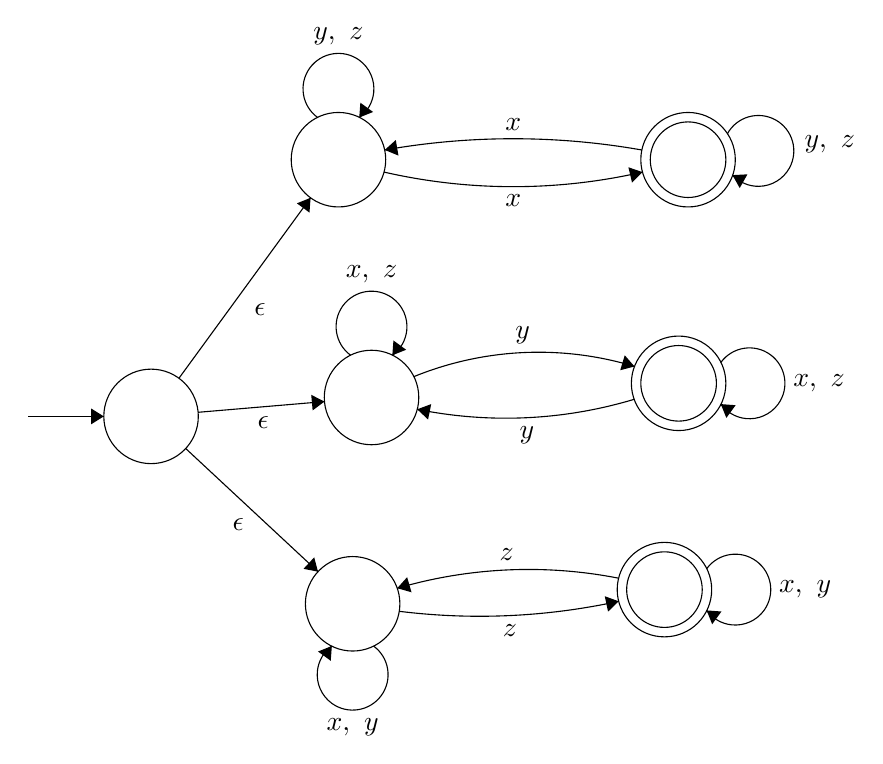
\begin{tikzpicture}[scale=0.2]
\tikzstyle{every node}+=[inner sep=0pt]
\draw [black] (16.5,-28.6) circle (3);
\draw [black] (28.4,-12.3) circle (3);
\draw [black] (29.3,-40.5) circle (3);
\draw [black] (50.6,-12.3) circle (3);
\draw [black] (50.6,-12.3) circle (2.4);
\draw [black] (49.1,-39.6) circle (3);
\draw [black] (49.1,-39.6) circle (2.4);
\draw [black] (30.5,-27.4) circle (3);
\draw [black] (50,-26.5) circle (3);
\draw [black] (50,-26.5) circle (2.4);
\draw [black] (8.7,-28.6) -- (13.5,-28.6);
\fill [black] (13.5,-28.6) -- (12.7,-28.1) -- (12.7,-29.1);
\draw [black] (18.27,-26.18) -- (26.63,-14.72);
\fill [black] (26.63,-14.72) -- (25.76,-15.07) -- (26.56,-15.66);
\draw (23.03,-21.83) node [right] {$\epsilon$};
\draw [black] (47.706,-13.087) arc (-77.12124:-102.87876:36.816);
\fill [black] (47.71,-13.09) -- (46.81,-12.78) -- (47.04,-13.75);
\draw (39.5,-14.51) node [below] {$x$};
\draw [black] (18.7,-30.64) -- (27.1,-38.46);
\fill [black] (27.1,-38.46) -- (26.86,-37.55) -- (26.18,-38.28);
\draw (22.03,-35.04) node [below] {$\epsilon$};
\draw [black] (46.194,-40.343) arc (-77.72838:-97.0665:41.52);
\fill [black] (46.19,-40.34) -- (45.31,-40.02) -- (45.52,-41);
\draw (39.29,-41.79) node [below] {$z$};
\draw [black] (30.623,-43.18) arc (54:-234:2.25);
\draw (29.3,-47.75) node [below] {$x,\mbox{ }y$};
\fill [black] (27.98,-43.18) -- (27.1,-43.53) -- (27.91,-44.12);
\draw [black] (27.077,-9.62) arc (234:-54:2.25);
\draw (28.4,-5.05) node [above] {$y,\mbox{ }z$};
\fill [black] (29.72,-9.62) -- (30.6,-9.27) -- (29.79,-8.68);
\draw [black] (32.132,-39.514) arc (106.30386:78.90127:29.707);
\fill [black] (32.13,-39.51) -- (33.04,-39.77) -- (32.76,-38.81);
\draw (39.08,-37.81) node [above] {$z$};
\draw [black] (31.336,-11.684) arc (100.016:79.984:46.943);
\fill [black] (31.34,-11.68) -- (32.21,-12.04) -- (32.04,-11.05);
\draw (39.5,-10.47) node [above] {$x$};
\draw [black] (53.095,-10.655) arc (151.12502:-136.87498:2.25);
\draw (57.97,-11.33) node [right] {$y,\mbox{ }z$};
\fill [black] (53.42,-13.28) -- (53.88,-14.1) -- (54.37,-13.23);
\draw [black] (51.78,-38.277) arc (144:-144:2.25);
\draw (56.35,-39.6) node [right] {$x,\mbox{ }y$};
\fill [black] (51.78,-40.92) -- (52.13,-41.8) -- (52.72,-40.99);
\draw [black] (19.49,-28.34) -- (27.51,-27.66);
\fill [black] (27.51,-27.66) -- (26.67,-27.23) -- (26.76,-28.22);
\draw (23.62,-28.56) node [below] {$\epsilon$};
\draw [black] (33.188,-26.075) arc (112.15159:73.1335:21.002);
\fill [black] (47.2,-25.43) -- (46.58,-24.72) -- (46.29,-25.67);
\draw (40.1,-24.01) node [above] {$y$};
\draw [black] (52.68,-25.177) arc (144:-144:2.25);
\draw (57.25,-26.5) node [right] {$x,\mbox{ }z$};
\fill [black] (52.68,-27.82) -- (53.03,-28.7) -- (53.62,-27.89);
\draw [black] (29.177,-24.72) arc (234:-54:2.25);
\draw (30.5,-20.15) node [above] {$x,\mbox{ }z$};
\fill [black] (31.82,-24.72) -- (32.7,-24.37) -- (31.89,-23.78);
\draw [black] (47.179,-27.515) arc (-73.24831:-101.4666:28.285);
\fill [black] (33.4,-28.15) -- (34.09,-28.8) -- (34.29,-27.82);
\draw (40.37,-29.23) node [below] {$y$};
\end{tikzpicture} \\
$L_{2}$ is all strings over the alphabet $\Sigma = \{x, y, z\}$ where either $x$ or $y$ or $z$ occurs an odd number of times.
\end{center}

\section{Determine whether or not the following languages are regular.}
\begin{itemize}
\item $L_{1}$ is not a regular language as it is not possible to keep track of balancing of parentheses using regular expressions. This needs to be done with something like a stack.
\item $L_{2}$ is a regular language as the number of unique words inside the book is finite. This could be done with a regular expression by ORing all the words.
\item $L_{3}$ is also a regular language as the number of 10-digit prime numbers is limited. 
\item $L_{4}$ is not regular as it is the set of valid Ocaml programs. But there exists other languages (invalid programs with just random combination of keywords) over the alphabet so it is not regular. On the other hand, there is no regular expression that is capable of expressing the language.
\end{itemize}

\section{Give one advantage and one disadvantage of system described in Backus' \textit{speedcoding} paper}
\textit{Speedcoding} is good for its simplicity. It makes programming easy as it provides convenient input-output operations. However, data and instructions are handled using different forms which may seem a little counter intuitive. Also, the performance is another weakness of the system.

\end{document}